\documentclass{article}
\usepackage{a4wide}
\usepackage{graphicx}
\usepackage{amsmath, amsthm, amssymb}
\usepackage[utf8]{inputenc}
\usepackage{ngerman}
\usepackage{url}
\usepackage[ruled,vlined]{algorithm2e}
\usepackage{hyperref}
\usepackage{listings}

\newtheorem{thm}{Theorem}[section]
\newtheorem{cor}[thm]{Korollar}
\newtheorem{lem}[thm]{Lemma}
\newtheorem{defi}[thm]{Definition}
\usepackage{listings}
\lstdefinelanguage{Pseudo}{
  morekeywords={forall,if,then,else,return,while,do,for,DFS},
  sensitive=false,
  morecomment=[l]{//},
  morestring=[b]"
}


\begin{document}
\title{Einführung in die Technische Informatik (ETI)}
\date{Wintersemester 2025/26}
\author{Universität Stuttgart}
\maketitle
\tableofcontents

\newpage
\section{Boolean Algebra}
It is defined as a 3-tuple $(A, +, \cdot)$, where:

\begin{itemize}
  \item $A$: a set of elements
  \item $+, \cdot$: binary operations $A \times A \rightarrow A$
\end{itemize}

This tuple satisfies the following axioms for all $x, y, z \in A$:

\begin{enumerate}
  \item \textbf{Commutative:} $x \cdot y = y \cdot x$ and $x + y = y + x$
  \item \textbf{Distributive:} $x \cdot (y + z) = (x \cdot y) + (x \cdot z)$, and analogously for $+$
  \item \textbf{Neutral Elements:} $x \cdot 1 = x$, \; $x + 0 = x$
  \item \textbf{Inverse Elements:} $x \cdot \overline{x} = 0$, \; $x + \overline{x} = 1$
\end{enumerate}

\subsection*{Derived Theorems}
\begin{enumerate}
  \item \textbf{Elimination:} $x \cdot 0 = 0$, \; $x + 1 = 1$
  \item \textbf{Absorption:} $x \cdot (x + y) = x$, \; $x + (x \cdot y) = x$
  \item \textbf{Associativity:} $(x \cdot y) \cdot z = x \cdot (y \cdot z)$, and analogously for $+$
  \item \textbf{Idempotence:} $x \cdot x = x$, \; $x + x = x$
  \item \textbf{Double Negation:} $\overline{\overline{x}} = x$
  \item \textbf{De Morgan:} $\overline{(x + y)} = \overline{x} \cdot \overline{y}$ and $\overline{(x \cdot y)} = \overline{x} + \overline{y}$
\end{enumerate}

\section{VHDL Logic Operators}
VHDL is a hardware description language used to model and implement digital systems.

The expression \texttt{F <= X and Y;} assigns to \texttt{F} the result of the logical \texttt{and} between \texttt{X} and \texttt{Y}.

\begin{center}
\begin{tabular}{ |c|c| } 
 \hline
 Logical Operator & Example in VHDL \\ 
 \hline
 not & \texttt{F <= not X;} \\ 
 \hline
 and & \texttt{F <= X and Y;} \\ 
 \hline
\end{tabular}
\end{center}

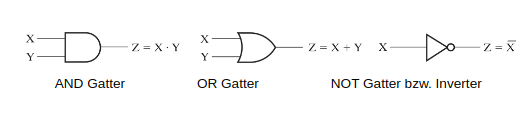
\includegraphics[]{assets/LogicGatesDrawing.png}

For example, a \textbf{NAND} gate is an AND gate with a negation bubble on the output.  
An \textbf{XOR} gate is an OR gate with an additional curved input line.  
An \textbf{XNOR} gate is the XOR gate with an output bubble (inverted output).

\section{CMOS Logic}
CMOS (\textit{Complementary Metal-Oxide-Semiconductor}) technology uses both N-channel and P-channel MOS transistors.

\begin{itemize}
  \item \textbf{N-channel (NMOS):} conducts when the input voltage is HIGH; open (non-conducting) when LOW.
  \item \textbf{P-channel (PMOS):} conducts when the input voltage is LOW; open (non-conducting) when HIGH.
\end{itemize}

A CMOS gate consists of:
\begin{itemize}
  \item a \textbf{Pull-Up Network (PUN)} made of PMOS transistors connected to $V_{DD}$
  \item a \textbf{Pull-Down Network (PDN)} made of NMOS transistors connected to GND
\end{itemize}

The goal is:
\begin{itemize}
  \item when $f(a,b,\dots)=1$, the output connects to $V_{DD}$ through the PUN,
  \item when $f(a,b,\dots)=0$, the output connects to GND through the PDN.
\end{itemize}

These networks are complementary:
\[
f_n = \overline{f(a,b,\dots)}, \qquad f_p = \overline{f_n(a,b,\dots)} = f(a,b,\dots)
\]

The fundamental CMOS gates are \textbf{NAND} and \textbf{NOR}; all other gates can be built from them and inverters.

\section{Definition of Important Terms}
\begin{itemize}
  \item \textbf{Disjunctive Normal Form (DNF):} e.g. $abc + bcd + cde$
  \item \textbf{Conjunctive Normal Form (CNF / KNF):} e.g. $(a+b+c)(b+d+e)$
  \item \textbf{Product Term:} conjunction of literals (negations allowed)
  \item \textbf{Sum Term:} disjunction of literals (negations allowed)
  \item \textbf{Minterm:} product of all literals, each appearing exactly once; output = 1
  \item \textbf{Maxterm:} sum of all literals, each appearing exactly once; output = 0
\end{itemize}

\subsection{Karnaugh Diagrams}
Omitted for now; worth revisiting later.

\subsection{VHDL : Example}
\begin{lstlisting}
entity compare is
  port ( a_i , b_i : in std_logic_vector ( 7 downto 0 );
    eq_o : out std_llogic );
end compare;
architecture rtl of compare is
begin
  eq_o <= '1' when ( a_i = b_i ) else '0';
end rtl;
\end{lstlisting}
\section{Number representation}
\begin{itemize}
  \item Sticks: ||, ||||....
  \item Roman Numerals, II, VI, CXL
  \item Position-Based-Systems
\end{itemize}

\subsection{Position Based Systems}
We have a basis $B$, and some Digits $C_i: C_i \leq B-1, C_i \geq 0$

The value of number $Z = C_{n-1}\cdot B^{n-1} + \dots +C_1\cdot B^1 + C_0 \cdot B^0$

Binary system uses base 2, decimal system uses Base 10.

\subsection{Decimal to Binary}
Find the biggest power of 2 thats smaller than n, and subtract. Repeat until n = 0. The powers subtracted form the number.

Also possible by dividing by two and the rest is the value at that position, the coefficient is divided once again.

\subsection{Binary to HexaDecimal}
Grab the first 4 bits and convert to hexadecimal, repeat for the next 4 bits and so on. In case of remaining, just add zeroes.

\section{Arithmetical Operations (on binary)}
\subsection{Addition}
Its trivial, treat is as decimal addition but with the cap being 2 instead of 10.

\subsection{Subtraction}
Its also relatively trivial, the only trouble is with the representation of negative numbers
\subsection{Subtraction through Complement and Addition}

For a given subtraction $D = M - S$, we can rephrase it as:
\[
D = M + (K - S) - K
\]
The idea is to simplify subtraction by replacing it with addition, provided we follow some ground rules:

\begin{itemize}
  \item $K \geq S$
  \item $K - S$ should be easy to compute
  \item $K$ should be easy to subtract
\end{itemize}

To achieve this, we define two types of complements based on the number base $B$.

\subsubsection{(B-1) Complement}
The \textbf{(B-1) complement} of a number is obtained by subtracting each digit from $(B-1)$.

\begin{verbatim}
Example in base 10:
  Number:          352
  9's complement:  999 - 352 = 647

Example in base 2:
  Number:          10101
  1's complement:  invert all bits = 01010
\end{verbatim}

Mathematically:
\[
(B - 1)\text{-complement}(N) = (B^n - 1) - N
\]
where $n$ is the number of digits (or bits) in $N$.

\subsubsection{B's Complement}
The \textbf{B's complement} of a number is obtained by adding $1$ to its (B-1) complement.

\begin{verbatim}
Example in base 10:
  Number:           352
  9's complement:   647
  10's complement:  647 + 1 = 648

Example in base 2:
  Number:           10101
  1's complement:   01010
  2's complement:   01010 + 1 = 01011
\end{verbatim}

Mathematically:
\[
B\text{-complement}(N) = B^n - N = [(B - 1)^n - N] + 1
\]

\subsubsection{Using Complements for Subtraction}
To compute $M - S$ using complements:
\[
M - S = M + (\text{B's complement of } S)
\]
If there is an overflow (a carry beyond $n$ digits), discard it.

\begin{verbatim}
Example in base 10 (10's complement):
  M = 352, S = 127
  10's complement of 127 = 873
  M + (10's complement of S) = 352 + 873 = 1225
  Discard overflow '1' → Result = 225
\end{verbatim}

\subsubsection{Representation of Negative Numbers}
In digital systems, complements are also used to represent \textbf{negative numbers}.

\paragraph{1's Complement (Binary)}
A negative number is represented by inverting all bits of its positive value.
\[
- N = \text{1's complement of } N
\]
Example:
\begin{verbatim}
+5 = 0101
-5 = 1010   (1's complement)
\end{verbatim}

However, this causes the issue of having both \texttt{+0 = 0000} and \texttt{-0 = 1111}, 
so it is rarely used in hardware.

\paragraph{2's Complement (Binary)}
In the \textbf{2’s complement system}, a negative number is represented by taking the 
1’s complement and adding 1:
\[
- N = (\text{2's complement of } N)
\]
Example:
\begin{verbatim}
+5 = 0101
1's complement = 1010
Add 1 → 1011
So, -5 = 1011 = -2*10^3 + 2 * 10^1 + 2*10^0 = -8 + 2 + 1 = -5 
\end{verbatim}



Advantages of 2's complement:
\begin{itemize}
  \item Only one representation of zero.
  \item Addition and subtraction use the same circuit.
  \item The most significant bit (MSB) acts as a sign bit (0 = positive, 1 = negative).
  \item To convert the number to decimal, the leftmost digit is negative and the rest are positive.
\end{itemize}

Thus, subtraction such as $M - S$ can be done by:
\[
M - S = M + (\text{2's complement of } S)
\]
and any overflow bit is discarded automatically.

\subsection{Multiplication}
Treat it exactly as a decimal multiplication. First digit * the number, then second digit * number * 10(one shift) and so on
\section{Binary Codes – Numerical Codes}

\subsection{Binary Code}
A \textbf{binary code} is a group of $n$ bits that can represent $2^n$ different combinations of 0s and 1s.  
Each unique bit pattern corresponds to a specific encoded element, such as a number or character.

\paragraph{Example: Binary Coded Decimal (BCD)}
In \textbf{BCD}, each decimal digit (0–9) is represented by its own 4-bit binary code.

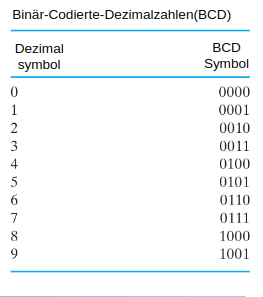
\includegraphics[]{assets/BCD.png}

This makes conversions between decimal and binary systems straightforward, although it is less space-efficient than pure binary representation.

\subsection{Dual Code}
The \textbf{dual code} (or \textbf{binary positional code}) is a standard binary representation in which each bit position has a weight of a power of 2.  
The numeric value of a code word is obtained by summing all the bit weights that are set to 1.

\[
\text{Example: } (1011)_2 = 1\cdot2^3 + 0\cdot2^2 + 1\cdot2^1 + 1\cdot2^0 = 11_{10}
\]

This is the most common numeric code used in computers for arithmetic and logic operations.

\subsection{Gray Code}
\textbf{Gray code} is a binary code designed so that consecutive numbers differ by only \textbf{one bit}.  
This property minimizes errors in systems where signals change gradually (e.g., rotary encoders, analog-to-digital converters).

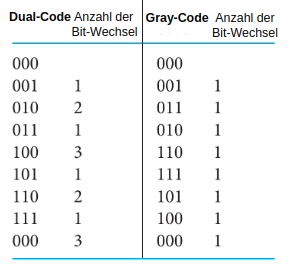
\includegraphics[]{assets/graycode.png}

Because only one bit changes at a time, Gray code reduces the chance of misreading during transitions between states.  
It was used extensively in older hardware systems and remains relevant in error-sensitive applications.

\section{Binary Codes – Alphanumerical Codes}

\subsection{ASCII Code}
The \textbf{American Standard Code for Information Interchange (ASCII)} is a 7-bit character encoding system that defines 128 possible symbols.

\begin{itemize}
  \item 94 characters are printable (letters, digits, punctuation, etc.)
  \item 34 are control characters (e.g., \texttt{Enter}, \texttt{Tab}, \texttt{Backspace})
\end{itemize}

\[
\text{Example: } 'A' = 65_{10} = 1000001_2
\]

ASCII became the foundation for most modern text encodings and is still embedded within larger standards like Unicode.

\subsection{Unicode}
Because ASCII’s 128-symbol limit is insufficient for all global alphabets, the \textbf{Unicode standard} was developed.

Unicode assigns a unique \textbf{code point} to every character in nearly all writing systems, symbols, and emojis.  
It supports over \textbf{1,000,000} possible code points.

Modern implementations typically use \textbf{UTF-8}, \textbf{UTF-16}, or \textbf{UTF-32} to store these code points efficiently.

\section{Binary Operations on a Hardware Level}

\subsection{Half Adder (HA)}
A \textbf{Half Adder} is a combinational circuit that takes two binary inputs $a$ and $b$, and produces two outputs: the \textit{sum} ($s$) and the \textit{carry} ($c$). The sum represents $a + b$, while the carry indicates overflow when both inputs are $1$.

\begin{center}
\begin{tabular}{ |c|c|c|c| } 
 \hline
 a & b & c & s  \\ 
 \hline
 0 & 0 & 0 & 0 \\ 
 0 & 1 & 0 & 1 \\ 
 1 & 0 & 0 & 1 \\ 
 1 & 1 & 1 & 0 \\ 
 \hline
\end{tabular}
\end{center}

It can be realized using logic gates as follows:
\begin{itemize}
  \item $c \leftarrow a \land b$
  \item $s \leftarrow a \oplus b$
\end{itemize}

\subsection{Full Adder (FA)}
A \textbf{Full Adder} extends the functionality of the Half Adder by including a third input $d$, representing the carry from the previous digit. It produces a sum $s$ and a carry $c$.

\begin{center}
\begin{tabular}{ |c|c|c|c|c| } 
 \hline
 a & b & d & c & s  \\ 
 \hline
 0 & 0 & 0 & 0 & 0 \\ 
 0 & 0 & 1 & 0 & 1 \\ 
 0 & 1 & 0 & 0 & 1 \\ 
 0 & 1 & 1 & 1 & 0 \\ 
 1 & 0 & 0 & 0 & 1 \\ 
 1 & 0 & 1 & 1 & 0 \\ 
 1 & 1 & 0 & 1 & 0 \\ 
 1 & 1 & 1 & 1 & 1 \\ 
 \hline
\end{tabular}
\end{center}

The logical computation is given by:
\begin{itemize}
  \item $s \leftarrow a \oplus b \oplus d$
  \item $c \leftarrow (a \land b) \lor (a \land d) \lor (b \land d)$
\end{itemize}

Since the full adder is essential for arithmetic operations and a traditional implementation uses around 40 transistors, efforts have been made to reduce transistor count.

A key simplification arises from observing that $s$ is typically the inverse of $c$, except in the cases where all inputs are either $1$ or $0$. Thus:

\[
s_i = (a_i + b_i + d_i) \cdot \overline{c_i} + a_i \cdot b_i \cdot d_i
\]

This optimized implementation requires fewer transistors.

\begin{center}
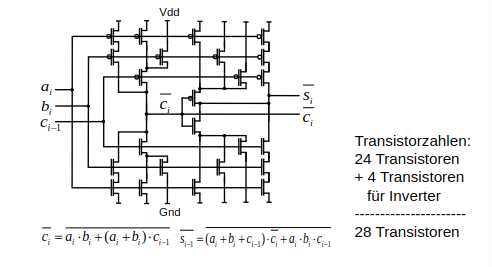
\includegraphics[scale=0.5]{assets/volladierer.png}
\end{center}

\subsection{Ripple Carry Adder}
A \textbf{Ripple Carry Adder} connects multiple full adders in sequence so that the carry output of one adder becomes the carry input of the next.

VHDL code for a 4-bit ripple carry adder:
\begin{lstlisting}
entity ripple_carry_adder is
  port (
    A  : in  std_logic_vector (3 downto 0);
    B  : in  std_logic_vector (3 downto 0);
    C0 : in  std_logic;
    S  : out std_logic_vector(3 downto 0);
    C4 : out std_logic
  );
end entity ripple_carry_adder;

architecture structure of ripple_carry_adder is
  signal C : std_logic_vector(4 downto 0);
begin
  C(0) <= C0;

  ripple_adder_generation : for i in 0 to 3 generate
    full_adder_I : entity work.full_adder
      port map (
        A    => A(i),
        B    => B(i),
        Cin  => C(i),
        Cout => C(i+1),
        S    => S(i)
      );
  end generate ripple_adder_generation;

  C4 <= C(4);
end architecture structure;
\end{lstlisting}

\textit{Note:} A cleaner version of this VHDL code can be found in VL~4, Teil~2, page~15.

\subsection{Binary Adder and Subtractor}
By adding an extra input $S$, the circuit can function as both an adder and a subtractor:
\begin{itemize}
  \item $S = 0$: performs addition.
  \item $S = 1$: performs subtraction.
\end{itemize}

For each input $B_i$, the value is XORed with $S$ before entering the full adder:
\[
B_i' = B_i \oplus S
\]
If $S = 0$, $B_i'$ remains unchanged.  
If $S = 1$, $B_i'$ becomes $\overline{B_i}$, and by setting the initial carry input to $S$, the circuit adds $1$, effectively computing the two’s complement.

% ============================================================
\section{Floating Point Arithmetic}

\subsection{IEEE 754 Floating Point Standard}
According to the IEEE 754 standard, a floating-point number consists of three parts:
\begin{enumerate}
  \item \textbf{Sign bit:} The first bit; 1 represents negative, 0 represents positive.
  \item \textbf{Exponent with bias:} An 8-bit unsigned value. The true exponent is obtained by subtracting the bias (127).
  \item \textbf{Significand (Mantissa):} Represents the fractional part after the binary point. The integer part before the point is implicitly 1.
\end{enumerate}

\textbf{Example:}  
\[
1\ 10000011\ 01000000000000000000000
\]
\[
- 2^{131 - 127} \times (1.0100)_2 = -2^4 \times 1.25 = -20
\]

\subsubsection{Positive Zero}
All bits are zero; interpreted as $+0$. Represents the smallest possible positive number.

\subsubsection{Negative Zero}
All bits are zero except for the sign bit, which is 1; interpreted as $-0$.

\subsubsection{Infinities}
Exponent is all ones, significand all zeros. Represents positive or negative infinity depending on the sign bit.

\subsubsection{NaN – Not a Number}
Exponent is all ones, significand is non-zero. Represents an undefined numerical result.

\begin{center}
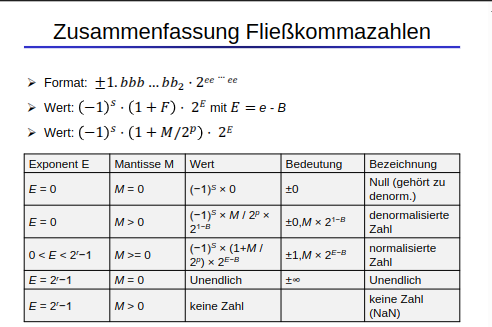
\includegraphics[scale=0.7]{assets/summaryFloatingPoint.png}
\end{center}

\subsection{Floating Point Addition and Subtraction}
\begin{enumerate}
  \item \textbf{Null checking:} If one operand is zero, return the other.
  \item \textbf{Exponent alignment:} Shift the significand of the smaller exponent to the right until both exponents match.
  \item \textbf{Addition/Subtraction:} Perform the arithmetic on the aligned significands. Watch for overflow.
  \item \textbf{Normalization:} Adjust the significand and exponent to maintain proper format.
  \item \textbf{Rounding:} Apply the appropriate rounding method.
\end{enumerate}

\subsubsection{Rounding Strategies}
\begin{center}
\begin{tabular}{ |c|p{5cm}| } 
 \hline
 \textbf{Rounding Strategy} & \textbf{Description} \\ 
 \hline
 Rounding towards zero & The result is truncated towards zero. \\ 
 \hline
 Rounding towards $\pm\infty$ & The result is rounded towards positive or negative infinity, depending on the sign. \\ 
 \hline
 Rounding to the nearest representable number & The result is rounded to the closest representable value. \\ 
 \hline
\end{tabular}
\end{center}

\subsection{Multiplication of Floating Point Numbers}
Floating-point multiplication is performed by:
\begin{enumerate}
  \item Adding the exponents (subtracting the bias if necessary),
  \item Multiplying the significands,
  \item Applying normalization and rounding.
\end{enumerate}

\section{Sequential Circuits}

\subsection{Dynamic Storage}
A single transistor can be used to temporarily store a bit of data.

\begin{center}
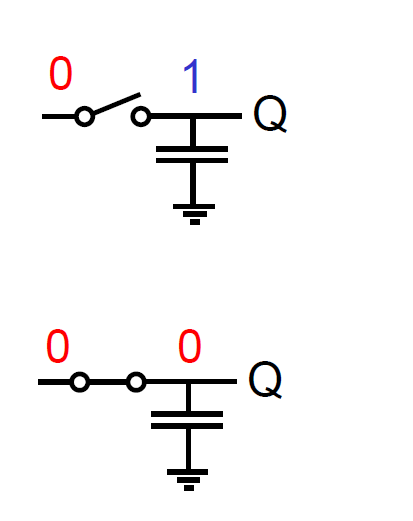
\includegraphics[scale=0.5]{assets/dynamicalstorage.PNG}
\end{center}

The main issue with this type of storage is that the stored voltage gradually decreases over time due to leakage currents and imperfect isolation. Therefore, it requires periodic refreshing.

\subsection{Static Storage}
A more reliable approach uses a \textbf{double inversion cycle}, where two inverters are connected in a feedback loop.

\begin{center}
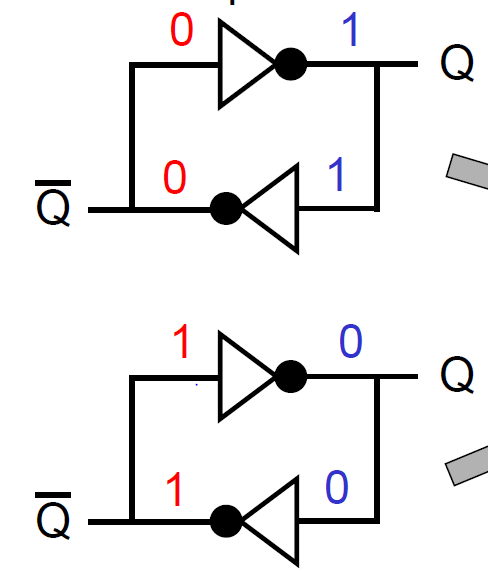
\includegraphics[scale=0.5]{assets/staticStorage.png}
\end{center}

This principle forms the basis of \textbf{latches} and \textbf{flip-flops}, which are fundamental building blocks of sequential logic.

\subsection{Latch with Set Input}
A latch can be extended with an additional input that forces the output $Q$ to 1 (and $\overline{Q}$ to 0).  
This input is called $\overline{S}$ (the active-low Set signal). When $S = 1$, then $\overline{S} = 0$ and $Q$ becomes 1.

\begin{center}
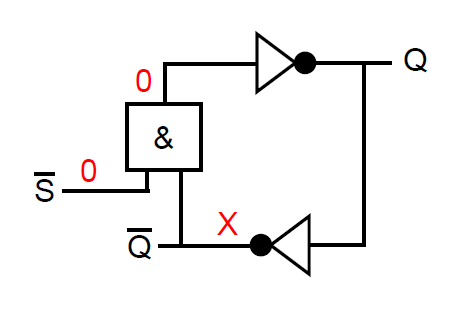
\includegraphics[scale=0.5]{assets/SetInputFlipFlop.PNG}
\end{center}

\subsection{Latch with Reset Input}
Similarly, a \textbf{reset input} allows the output $Q$ to be forced to 0.  
The corresponding signal is $\overline{R}$ (active-low Reset).

\subsection{RS Latch (Reset-Set Latch)}
The RS latch combines both the Set and Reset inputs.

\begin{center}
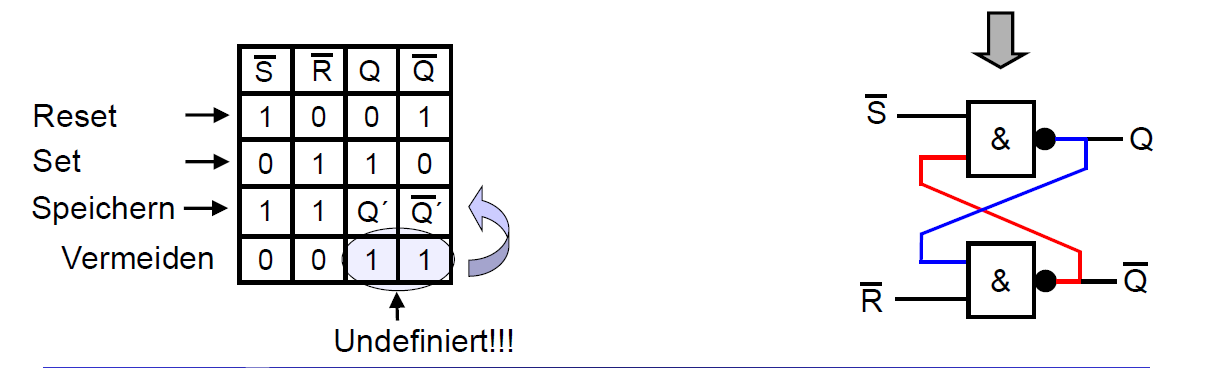
\includegraphics[scale=0.45]{assets/RSFlipFlop.PNG}
\end{center}

The behavior is as follows:
\begin{itemize}
    \item $S = 1$, $R = 0$: Set ($Q = 1$)
    \item $S = 0$, $R = 1$: Reset ($Q = 0$)
    \item $S = R = 1$: Hold (no change)
    \item $S = R = 0$: Undefined state
\end{itemize}

\begin{center}
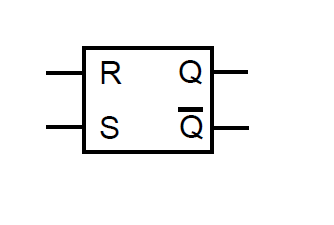
\includegraphics[scale=0.5]{assets/RSFlipFlopSymbol.PNG}
\end{center}

While the RS latch is useful, it does not take the clock signal into account, which limits its reliability in synchronous systems.  
However, it is still suitable for simple asynchronous tasks such as key debouncing or switch state storage.

\subsection{Gated SR Latch}
A gated SR latch introduces a \textbf{clock (enable)} signal $C$ that allows writing only when $C = 1$.

\begin{center}
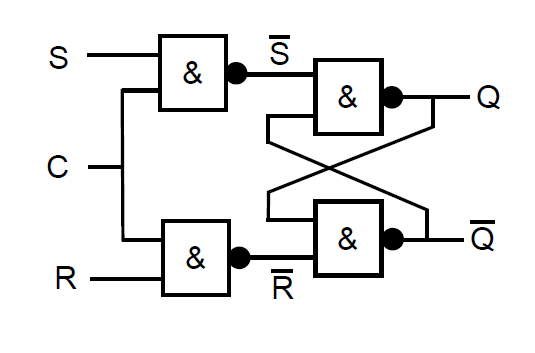
\includegraphics[scale=0.5]{assets/GatedSRLatch.png}
\end{center}

This implementation requires around 16 transistors.

\subsection{D Latch}
A simplified version of the SR latch is the \textbf{D latch}, which uses a single data input $D$ and defines:
\[
S := D, \qquad R := \overline{D}
\]

This design requires approximately 18 transistors.  
Alternatively, a D latch can also be implemented using multiplexers.

The drawback of a D latch is that it is \textbf{level-sensitive}—it is transparent when the clock is high, meaning input changes immediately propagate to the output.  
If data is written outside the intended clock phase, unwanted behavior can occur.  
To address this, a second D latch is used with an inverted clock signal ($C' = \overline{C}$).

\subsection{D Flip-Flop}
\begin{center}
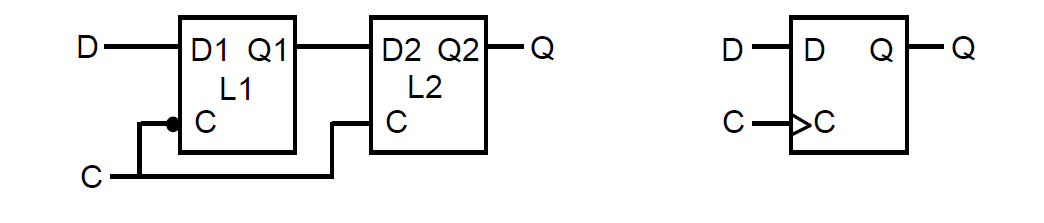
\includegraphics[scale=0.4]{assets/DFlipFlop.PNG}
\end{center}

A \textbf{D flip-flop} samples the input only at a specific clock transition (rising or falling edge), thus avoiding glitches and undefined intermediate voltages.

It can also be implemented using two D latches (a \textit{master–slave} configuration) or multiplexers.

\textbf{Issue:} If the input changes too close to a clock transition, unpredictable behavior may occur.  
\textbf{Solution:} Define \textit{setup} and \textit{hold} times.

\subsection{Setup and Hold Times in a D Flip-Flop}
The \textbf{setup time} ($t_{setup}$) is the minimum time before a clock edge during which the input data must remain stable.  
The \textbf{hold time} ($t_{hold}$) is the minimum time after the clock edge during which the input must continue to remain stable.  

\subsection{Static Timing Analysis (STA)}
\textbf{Static Timing Analysis} is a method used to determine the maximum operating frequency of a digital circuit without requiring simulation.  
It identifies the \textbf{longest propagation delay path} in the circuit — also known as the \textbf{critical path} — and uses it to calculate the highest possible clock frequency.

\subsubsection{Timing Graph}
A \textbf{timing graph} models a circuit as a directed graph where:
\begin{itemize}
    \item Each node represents a logic element (gate, flip-flop, etc.) with a delay.
    \item Each edge represents a connection
\end{itemize}

Nodes driven by a clock signal (e.g., the output of a flip-flop) are treated as \textbf{starting points} and therefore have no incoming edges, since they mark the beginning of a new clock cycle.

The goal of STA is to ensure that, for every path between two flip-flops, the data has enough time to propagate before the next clock edge.  
Formally, for correct operation, the following condition must hold for every path:
\[
t_{clk\_q} + t_{logic} + t_{setup} \leq T_{clk}
\]
where:
\begin{itemize}
    \item $t_{clk\_q}$ is the clock-to-output delay of the source flip-flop,
    \item $t_{logic}$ is the total propagation delay through the combinational logic,
    \item $t_{setup}$ is the setup time of the destination flip-flop,
    \item $T_{clk}$ is the clock period.
\end{itemize}

If this condition is violated, the clock frequency must be lowered until the inequality is satisfied.

\subsubsection{Pipelining}
\textbf{Pipelining} is a technique used to increase the maximum clock frequency by dividing a long combinational path into shorter segments.  
This is achieved by inserting \textbf{D flip-flops} between stages of the circuit.

Each flip-flop introduces a new clock boundary, effectively shortening the critical path delay for each stage:
\[
T_{clk}^{new} = \max(t_{stage1}, t_{stage2}, \ldots, t_{stagen})
\]

As a result, the circuit can operate at a higher clock speed, since each pipeline stage performs only a portion of the total computation per cycle.  
However, this also increases the \textbf{latency} (number of cycles required to complete a full operation) even though the \textbf{throughput} (operations per second) improves.

\section{Finite State Machines}

\subsection{Formal Definition}

A finite state transducer (FST) is defined as a 6-tuple
\[
(A, S, s_0, \delta, B, \lambda),
\]
where:
\begin{itemize}
  \item $A$: Finite set of input symbols (alphabet)
  \item $S$: Finite set of states
  \item $s_0 \in S$: Starting state
  \item $\delta : S \times A \to S$: State transition function
  \item $B$: Finite set of output symbols
  \item $\lambda$: Output function  
        \begin{itemize}
            \item Mealy type: $\lambda : S \times A \to B$
            \item Moore type: $\lambda : S \to B$
        \end{itemize}
\end{itemize}

\begin{center}
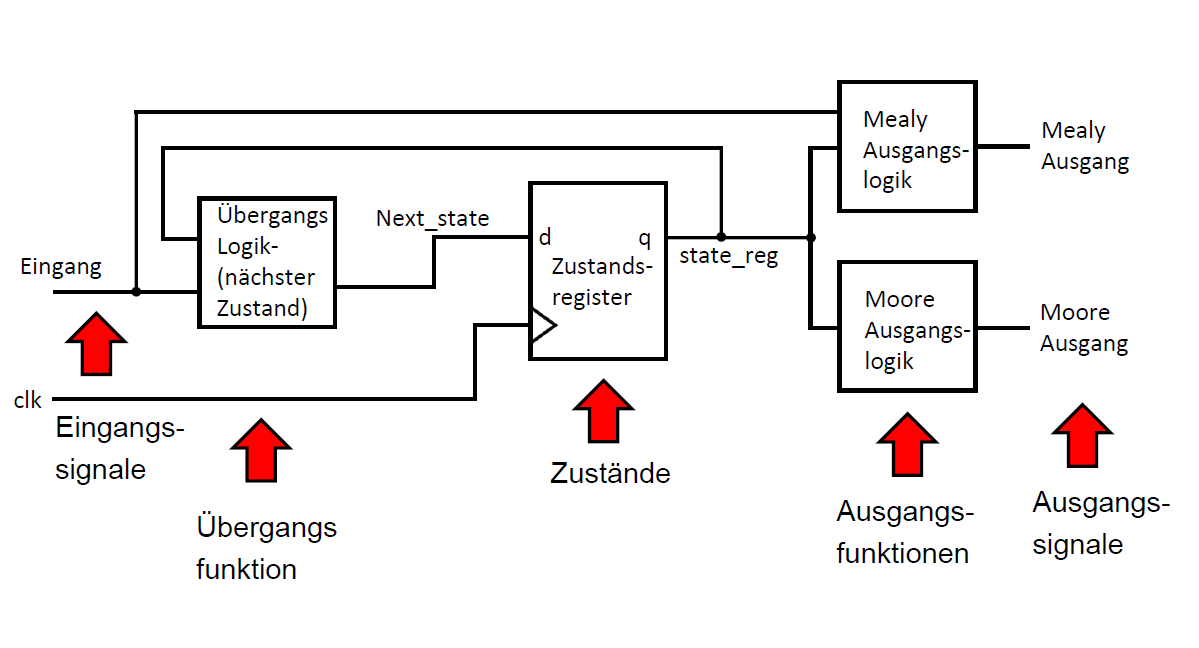
\includegraphics[scale=0.4]{assets/fst.PNG}
\end{center}

\subsection{Example: Traffic Light}

Consider a traffic light cycling through the states
\[
\text{green} \to \text{yellow} \to \text{red} \to \text{red+yellow} \to \text{green}.
\]

Rotating and encoding the light horizontally as binary gives:
\[
001 \to 010 \to 100 \to 110 \to 001.
\]

We represent the current state using a register of D-flip-flops.

\begin{center}
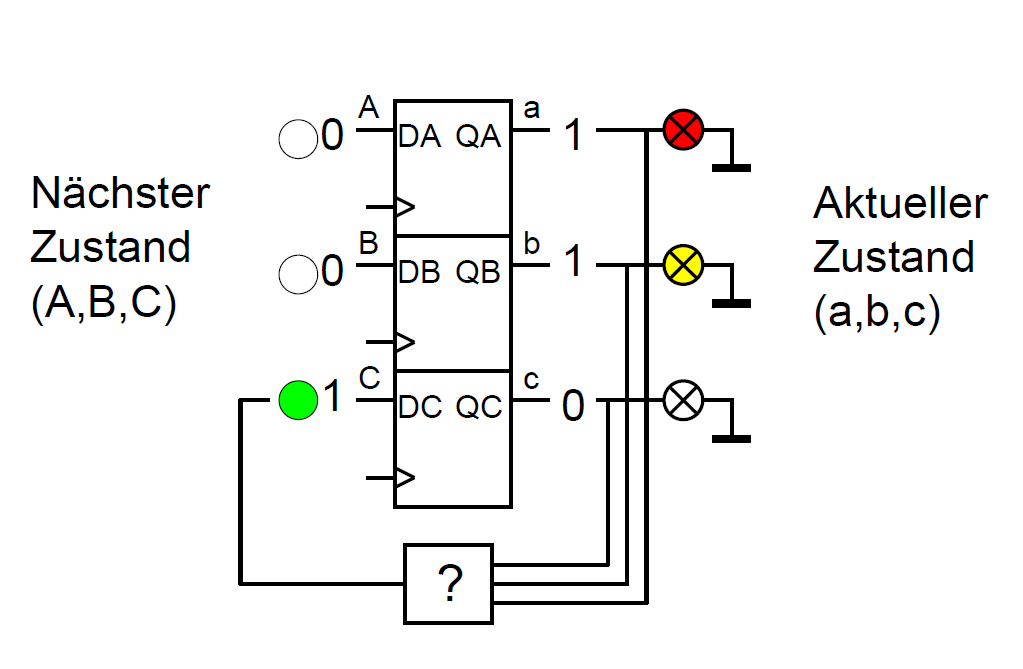
\includegraphics[scale=0.5]{assets/ampel.PNG}
\end{center}

We build a truth table for the transition logic:

\begin{center}
\begin{tabular}{|c|c|c||c|c|c|}
\hline
$a$ & $b$ & $c$ & $A$ & $B$ & $C$ \\
\hline
0 & 0 & 1 & 0 & 1 & 0 \\
0 & 1 & 0 & 1 & 0 & 0 \\
1 & 0 & 0 & 1 & 1 & 0 \\
1 & 1 & 0 & 0 & 0 & 1 \\
\hline
\end{tabular}
\end{center}

Resulting Boolean expressions:
\[
\begin{aligned}
C &= a b \bar{c}, \\
B &= \bar{a}\,\bar{b}\,c + a\bar{b}\,\bar{c}, \\
A &= \bar{a}\,b\bar{c} + a\bar{b}\,\bar{c}.
\end{aligned}
\]

\paragraph{Important Note}
It is essential to analyze how the system behaves under invalid input states.  
In this example, incorrect inputs would cause the system to cycle as:
\[
000 \to 000 \to 000 \dots
\]
which is harmless but must be known.

\subsection{Propagation Delay}

We define $\Delta$ as the delay of one logic gate.

Consider the logic function
\[
Z = \overline{\overline{b} + a}.
\]

We switch inputs from $(a,b)=(1,1)$ to $(0,0)$ and track the system over time.

\subsubsection*{Before the switch ($t < 0$)}
\begin{itemize}
    \item $a = 1$
    \item $b = 1$
    \item $\overline{b} = 0$
    \item $Z = \overline{0 + 1} = 0$
\end{itemize}

\subsubsection*{At the moment of switching ($t = 0$)}
\begin{itemize}
    \item $a = 0$
    \item $b = 0$
    \item $\overline{b} = 0$ (not updated yet)
    \item $Z = 0$ (not updated yet)
\end{itemize}

\subsubsection*{After one gate delay ($\Delta < t < 2\Delta$)}
\begin{itemize}
    \item $a = 0$
    \item $b = 0$
    \item $\overline{b} = 1$ (updated)
    \item $Z = 0$ (updated using old inputs)
\end{itemize}

\subsubsection*{After full settling ($t > 2\Delta$)}
\begin{itemize}
    \item $a = 0$
    \item $b = 0$
    \item $\overline{b} = 1$
    \item $Z = \overline{1 + 0} = 1$
\end{itemize}

This results in a temporary glitch of duration $\Delta$.  
In a traffic light controller, this would cause a brief flash of green after red.

\paragraph{Solution}
Place a D-flip-flop at the output to sample the value only after stabilization.

\section{SRAM and DRAM}

\subsection{RAM vs. Serial Memory}

\textbf{Random Access Memory (RAM)} provides constant access time for every address.

\textbf{Serial memory} (e.g., HDDs) has variable access time depending on mechanical factors such as disk rotation.

\paragraph{Word}
A \textbf{word} is a group of bits stored in a memory cell, typically a multiple of 8 bits (one byte).

\begin{center}
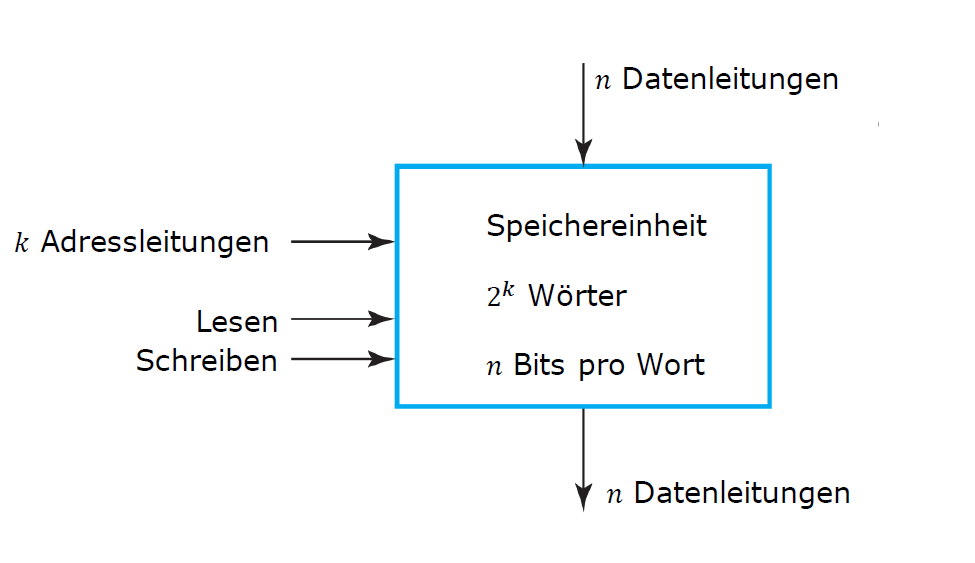
\includegraphics[scale=0.5]{assets/ram.PNG}
\end{center}

\subsubsection{Operations on RAM}
\begin{itemize}
    \item \textbf{Chip Select (CS)}:  
    A dedicated line enabling or disabling access to the chip (1 = active, 0 = inactive).
    \item \textbf{Read/Write}:  
    Determines the operation (0 = write, 1 = read).  
    Ignored when Chip Select is 0.
\end{itemize}

\subsection{SRAM — Static RAM}
\begin{itemize}
    \item Data is retained as long as power is supplied.
    \item Uses stable self-refreshing circuits (e.g., cross-coupled inverters).
    \item Faster than DRAM.
    \item Uses more physical area per bit.
\end{itemize}

\subsection{DRAM — Dynamic RAM}
\begin{itemize}
    \item Stores data in capacitors.  
    \item Values leak over time and must be periodically refreshed.
    \item Very compact: typically 1 transistor per bit.
\end{itemize}
\section{Designing a basic computer}
\subsection{Hardware architecture for a sum}
Lets say we want to compute 
\[y = \sum_{i=1}^{N = 10}a_i\]

We can just do a circuit with a register R0 that holds the current sum, and a register R1 that starts inputting the numbers in $a_i$. We just combine those two into an adder, and the output feeds back to R0.

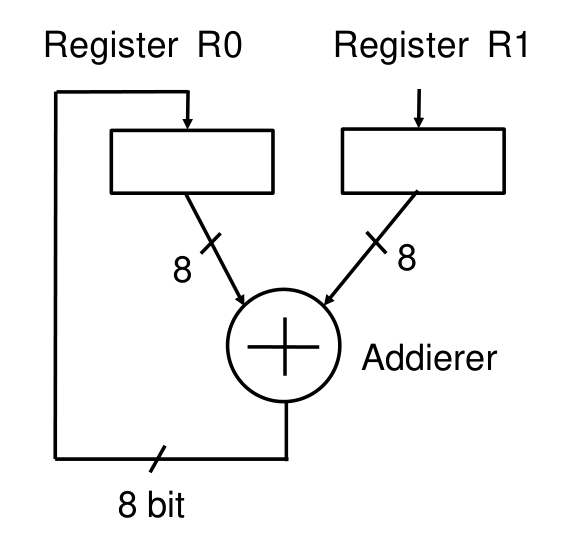
\includegraphics[scale=0.5]{assets/adder.PNG}

\subsection{Hardware architecture for basic operations}
We can use a third input C to determine the operation we wish to do.

Whenever we are able to handle all the basic operations, this is called an Arithmetic Logic Unit:  \textbf{ALU}

Basic operations with its C code
\begin{enumerate}
  \item 000 add
  \item 100 sub
  \item 010 mul
  \item 110 and
  \item 001 or
  \item 011 xor
\end{enumerate}

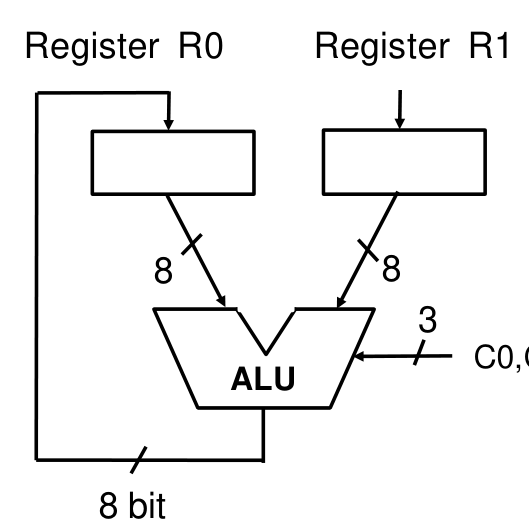
\includegraphics[scale=0.5]{assets/ALU.PNG}

Note: We also can switch the register R1 with a multiplexer and R1,..RN registers to allow all inputs from $a_1,..,a_n$

So now an instruction code will be

Operation Code (3 bits in this case) Register code (another 3 bits)

\subsection{Move - MOV}

Copies the contents of R0 into the set ADDRESS

\subsection{Jump - jmp}

Allows to jump within the assembly code.

MARK sub R2

...

jmp MARK

This code jumps back to MARK

\subsubsection{Conditional jumping - bnz}

This is a conditional jump if branch not zero, meaning if the previous operation is not zero it does the jump


\subsection{Clock speed of an ALU}
Given that the time delay of a full adder is around 50ps, the clock speed will be around 2.5GHz

\subsection{Types of computer architectures}
\subsubsection{Von-Neumann-Architecture}
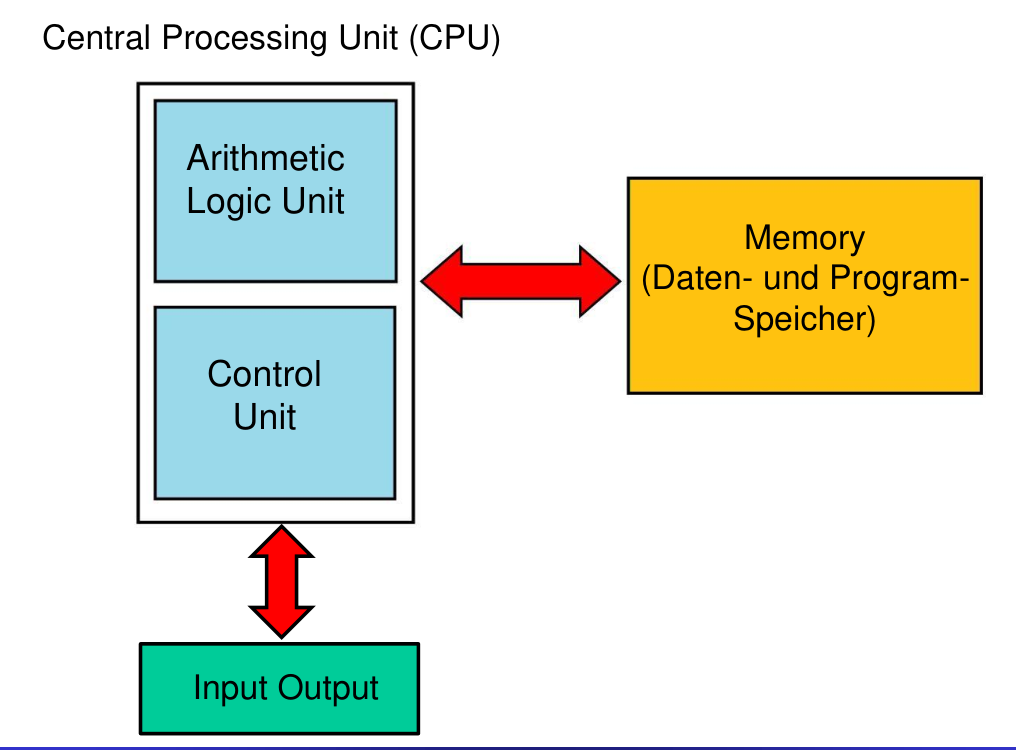
\includegraphics[scale=0.5]{assets/vonneumann.PNG}

The issue with this is that the storage is shared, so in theory the code could alter itself.

Another characteristic is that the words are of a set word length in this format

\subsubsection{Harvard Architecture}

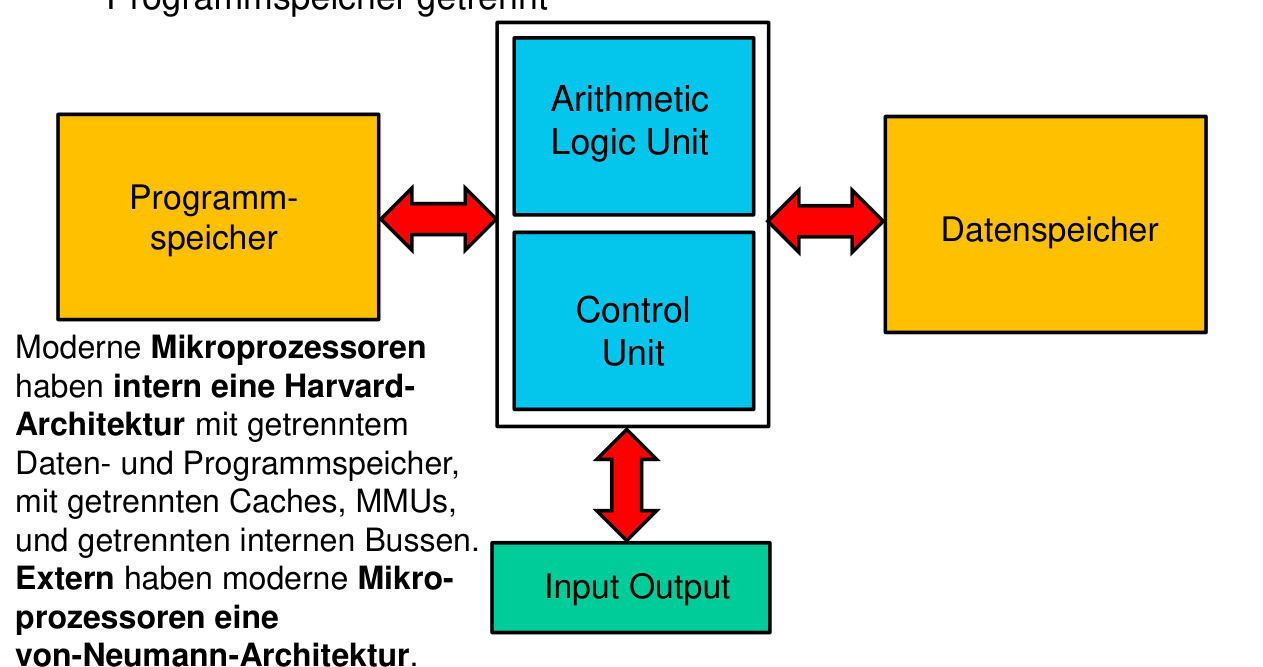
\includegraphics[scale=0.4]{assets/harvard.PNG}

Separated storage for programm and data, so no self altering.

\subsection{A computer architecture with an instruction set}

\subsubsection{Definition: Computer Architecture}
It can be defined as the description of the hardware at the block-diagramm level that explains the functionality of the system.

It can be divided in
\begin{itemize}
  \item Data Path
  \begin{itemize}
    \item ALU
    \item Control interface
    \item Register record
  \end{itemize}
  \item Control unit
  \begin{itemize}
    \item Provides signals based on the interpretation of commands
  \end{itemize}
\end{itemize}


\subsubsection{A typical data path}
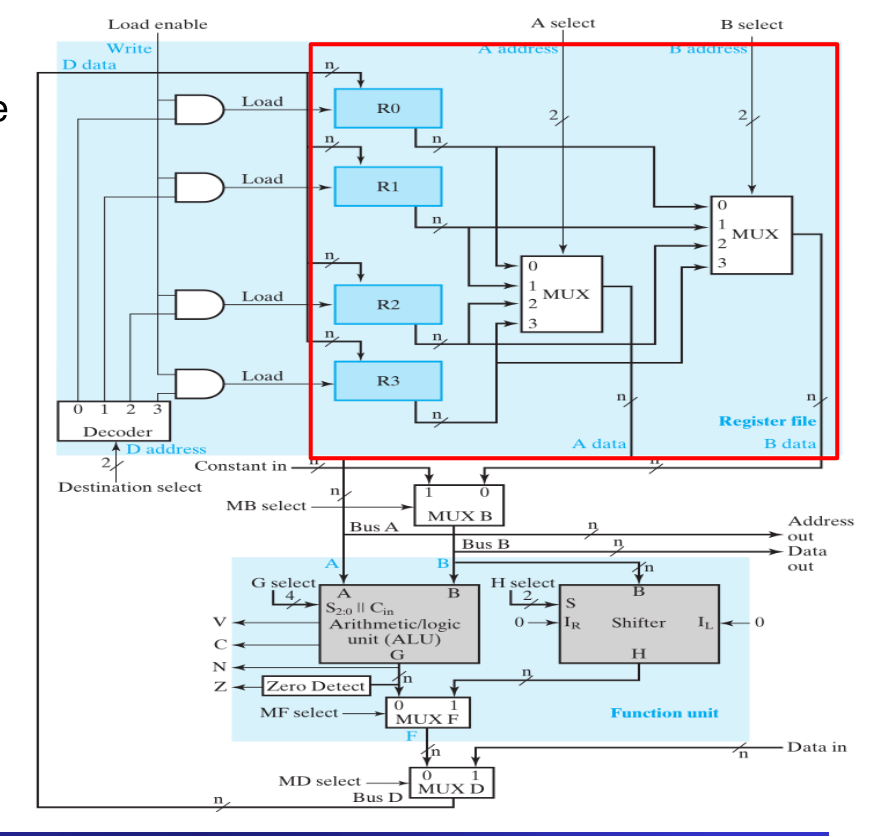
\includegraphics[scale=0.6]{assets/data_path.PNG}

\paragraph{Registers: }We have 4 registers in this case, with two multiplexers that allow us to select two of these registers. (A Select, B Select)

\paragraph{Bus A: }Its also connected to the external adress lines. Used for memory operations or I/O

\paragraph{Bus B: }Is connected to the data output. Used to send data to other components of the system that are not the data path

\paragraph{MUX B: } Allows to fill Bus B with a constant when set set to 1

\paragraph{ALU: }Used to do arithmetic + logic micro operations. Its inputs are the Buses A and B, with also an input called G-Select(4-bits) that selects the operation

It also contains some flags for extra info
\begin{itemize}
  \item Z : zero status - output = 0
  \item C : carry status - last carry digit = 1
  \item V : overflow status
  \item N : sign status
\end{itemize}


\paragraph{Shifter: } Used to shift bits left or right. Can only alter Bus B. 

\paragraph{MUX F: } Picks between the output of the shifter or the ALU

\paragraph{MUX D: } picks between the output of MUX F or external data. 

\paragraph{D Bus: }Contains the data line of the input for all registers.

\paragraph{Destination Select: } Picks which registers are filled and such with the data of the D-Bus

\subsubsection{Instruction execution}

Note: All this is done basically in parallel, but described as a list for easier understanding

Example: $R1 \leftarrow R2 + R3$
\begin{enumerate}
  \item A Select gets the value 2 to access R2
  \item B Select gets the value 3 to access R3
  \item G Select gets the value for the operation $A+B$
  \item MF-Select gets the value 0 to get the contents of the ALU
  \item MD-Select gets the value 0 to get the contents of the Data Path
  \item Destination Select picks R1 as the output Destination
  \item Load Enable is set to 1 to allow the data being written into R1
 
\end{enumerate}

\subsubsection{ALU - Deep Dive}
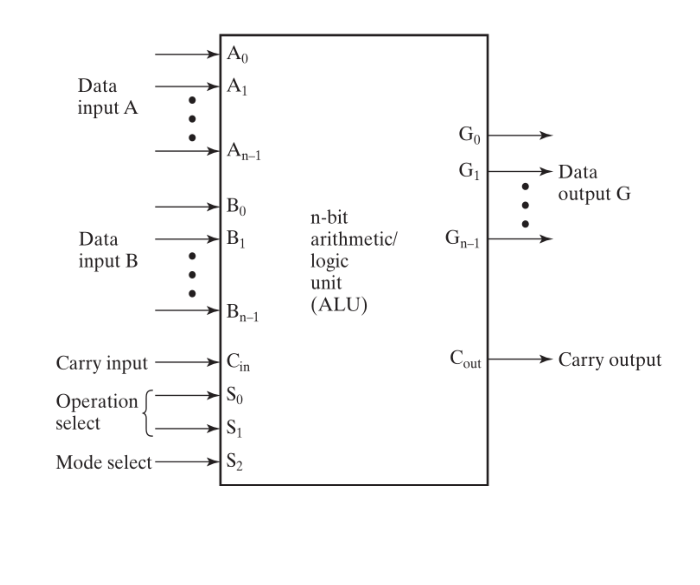
\includegraphics[scale=0.5]{assets/ALU2.png}

\paragraph{Operations on an ALU: }They are the following

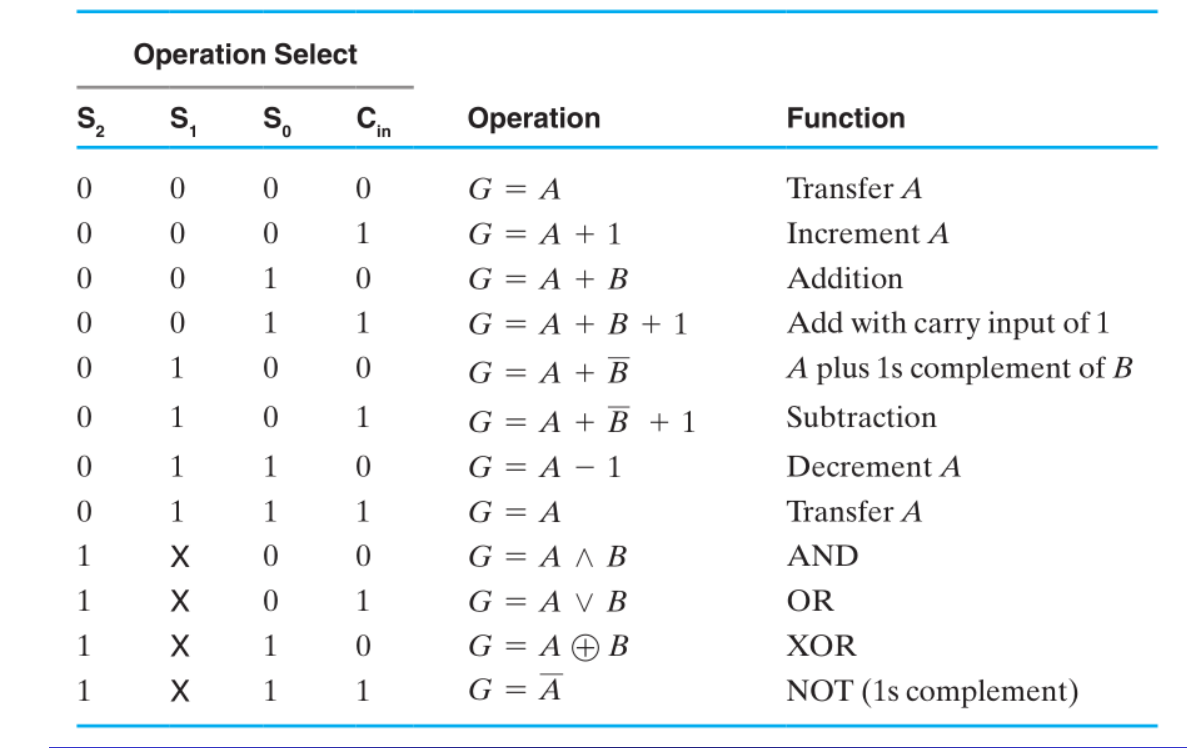
\includegraphics[scale=0.4]{assets/ALUOperations.png}

\subsubsection{Shifter}
The shifter handles shifting left or right the bits of Bus B. It consists of a series of multiplexers where each multiplexer i connects to $B_{i-1},B_i,B_{i+1}$. To pick the order of rotation. For the borders it contains $I_R,I,L$ as input values. To select the type of shift you use S.
\[\begin{cases}
  S = 00 & \text{ nothing}\\
  S = 01 & \text{ shift right once. } I_R \text{ is used}\\
  S = 10 & \text{ shift left once. } I_L \text{ is used}\\
\end{cases}\]

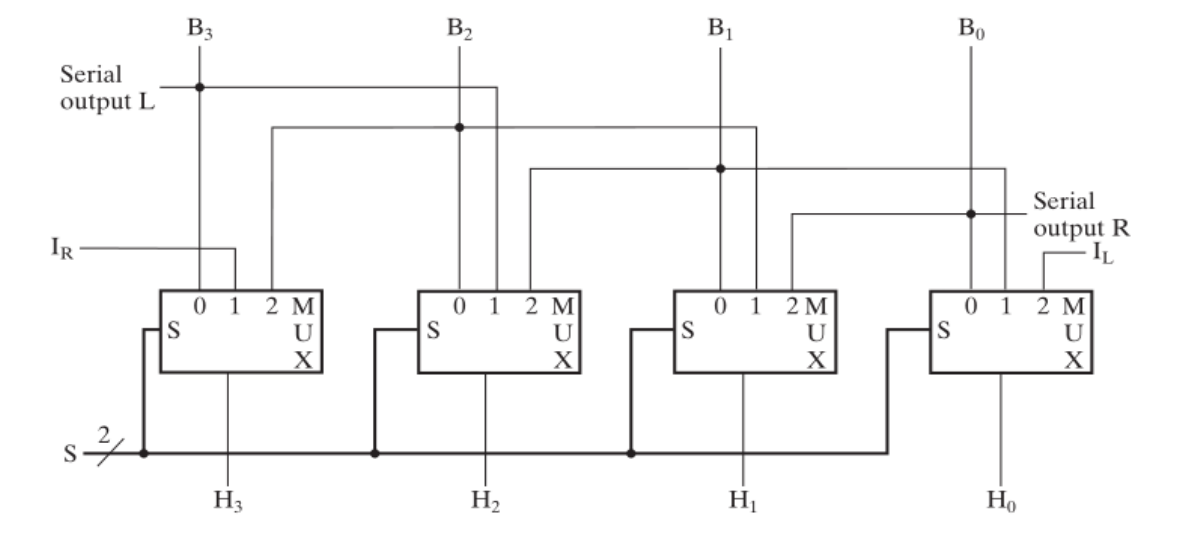
\includegraphics[scale=0.4]{assets/shifterç.png}

\subsubsection{Barrel Shifter}
Shifts n bit positions, defined by the binary value $(S_0,S_1)$

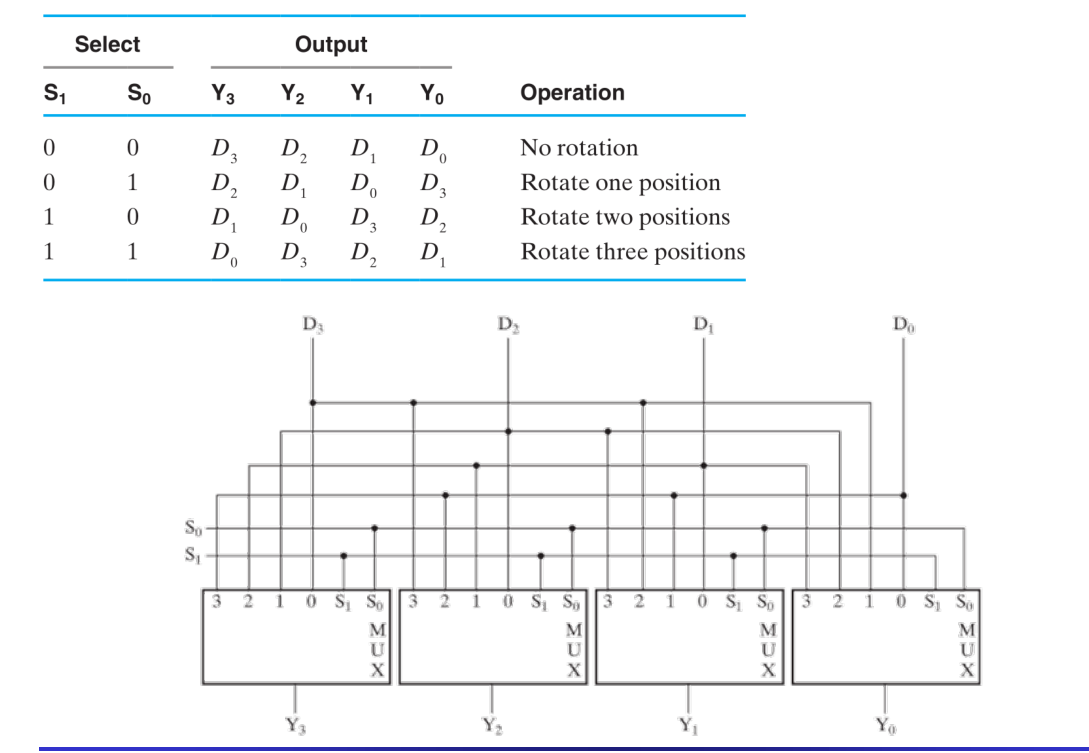
\includegraphics[scale=0.4]{assets/barrelshifter.png}

\subsubsection{Register File}
Its a fast storage comprised of registers. Allows reading/writing multiple words at at time.

m defines the amount of registers

n defines the amount of bits of the register

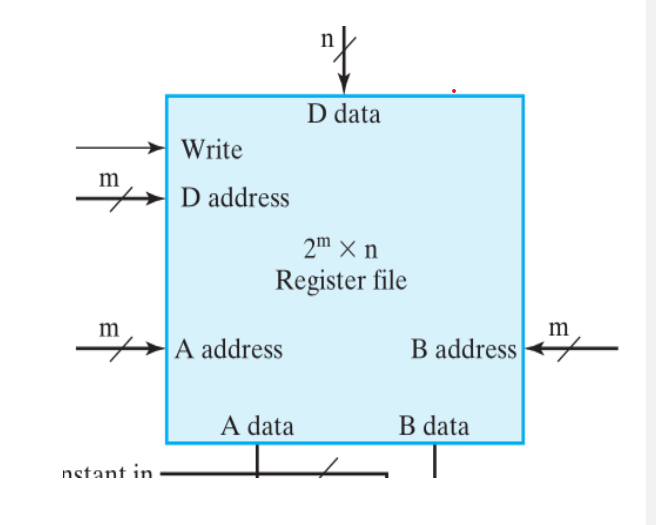
\includegraphics[scale=0.5]{assets/registerfiles.png}

The grabbing the data from the A, B and D adresses is all done in the same clock cycle.

\subsubsection{ALU + Shifter = Function Unit}
Values:
\begin{itemize}
  \item A,B inputs of the function
  \item F output
  \item V,C,N,Z statusbits described above
  \item  FS 4 bits Function Select
\end{itemize}
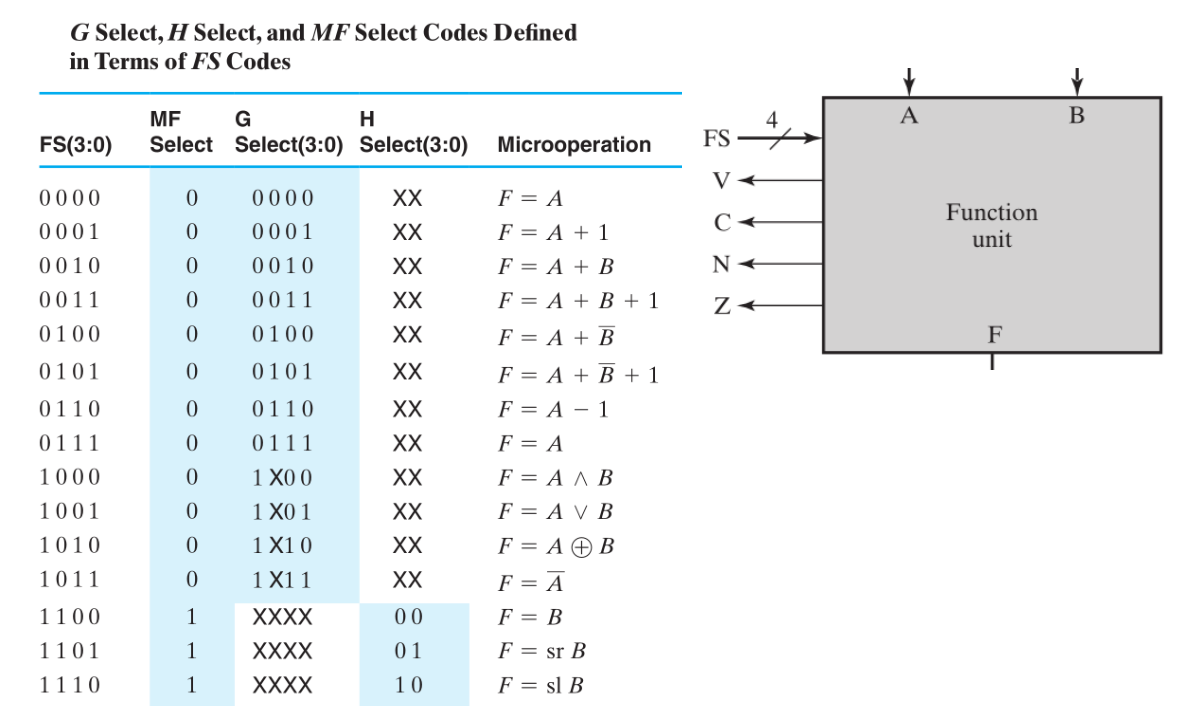
\includegraphics[scale=0.4]{assets/functionUnit.png}

\subsubsection{Control Word}
We use 16 bits to define a control word for our example

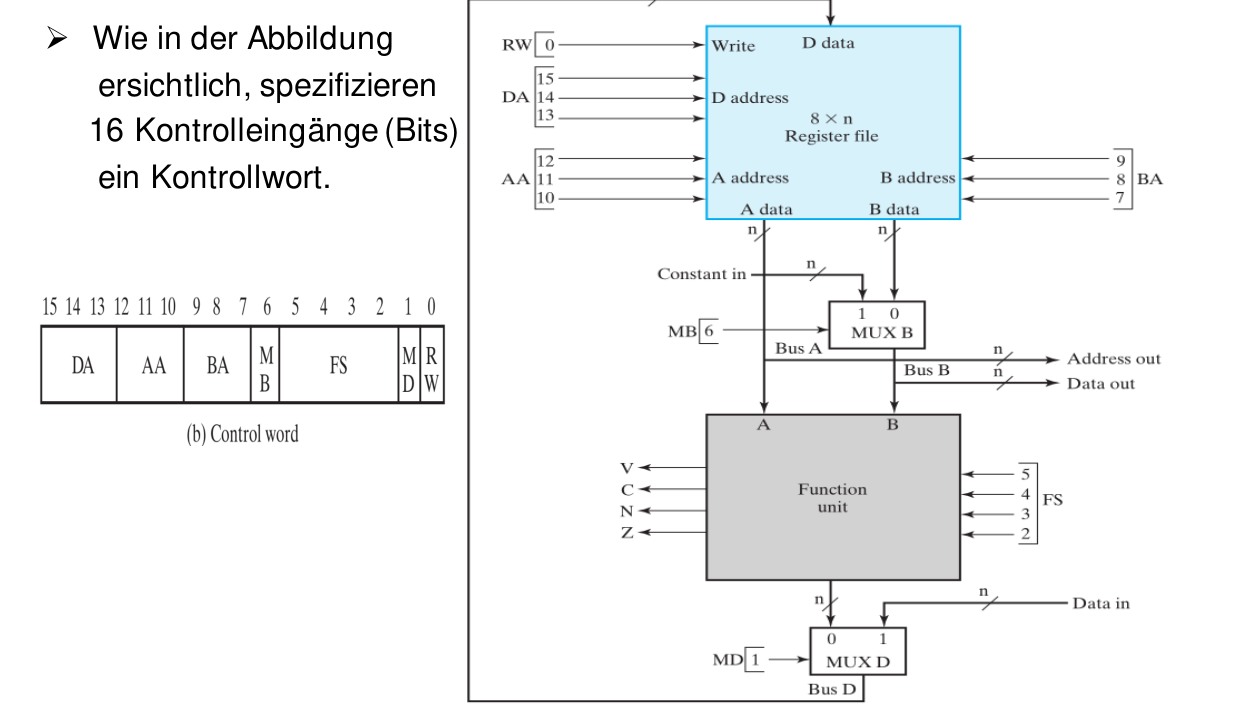
\includegraphics[scale=0.4]{assets/controlword.png}

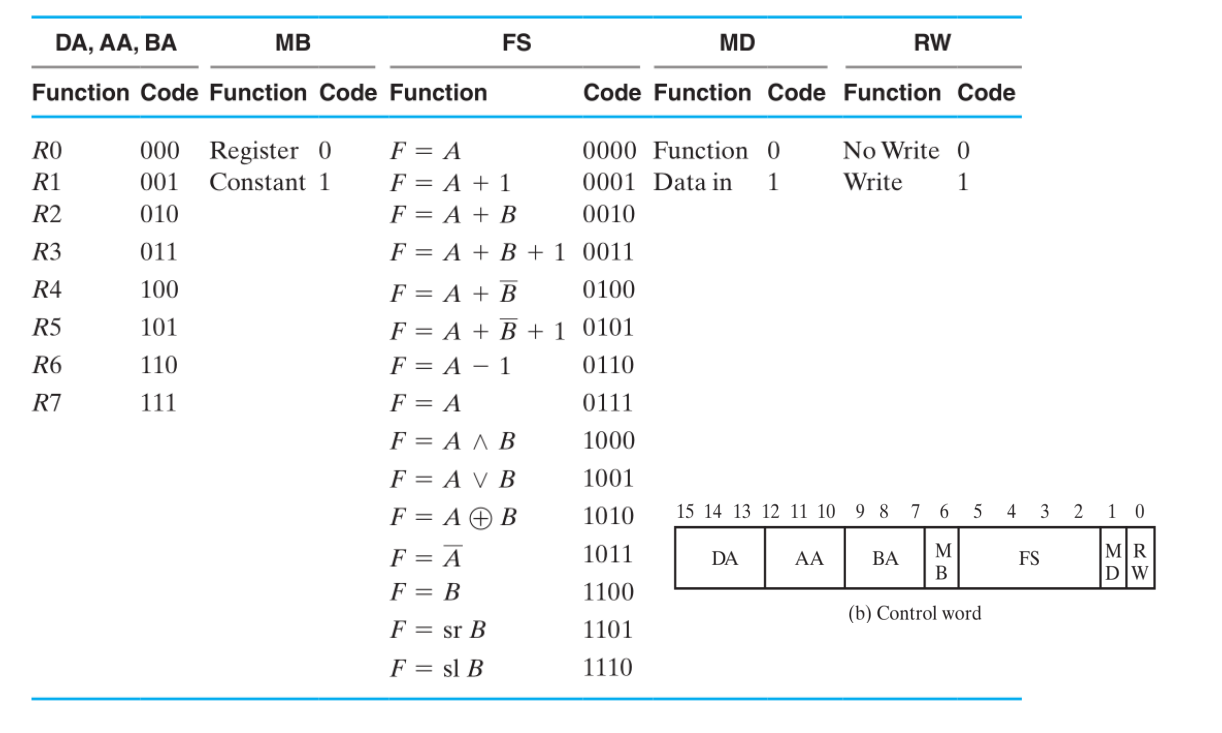
\includegraphics[scale=0.4]{assets/controlword1.png}

\subsubsection{Command format}
Usually represented throguh a bit group

Our format is as follows
\begin{itemize}
  \item Operation code: represents the operation to be done
  \item Destination register
  \item Source register A
  \item Source register B
\end{itemize}

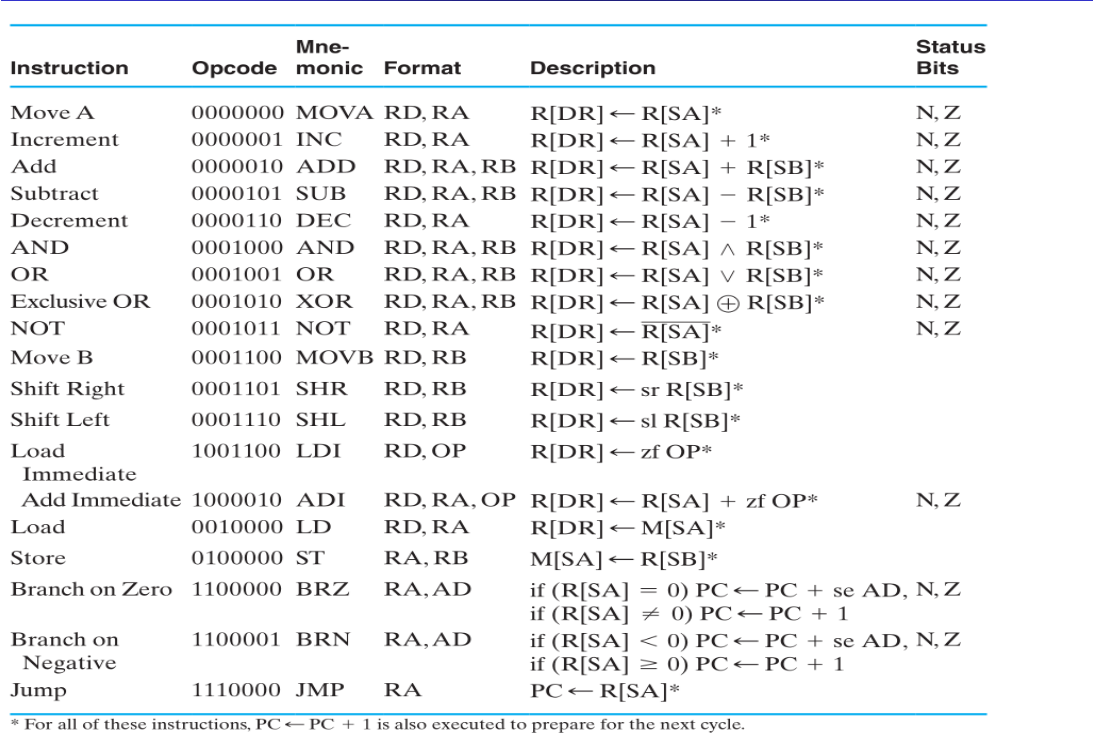
\includegraphics[scale=0.4]{assets/commandFormat.png}

\subsubsection{The Control Unit}
The computer delivers the command address to
the command memory. The output of the
command is then processed further in the decoder

\subsubsection{Instruction Decoder}
Combination of logic gates that provides all control words for the data path, based on the contents of the fields of the instruction.

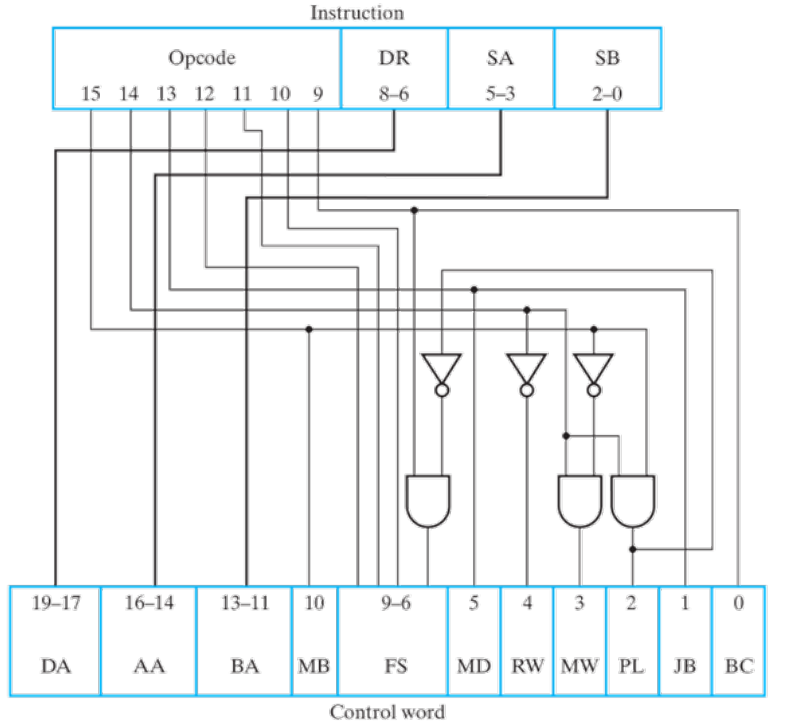
\includegraphics[scale=0.4]{assets/instructiondecoder.png}

\paragraph{Truth table for a Instruction Decoder: }Here

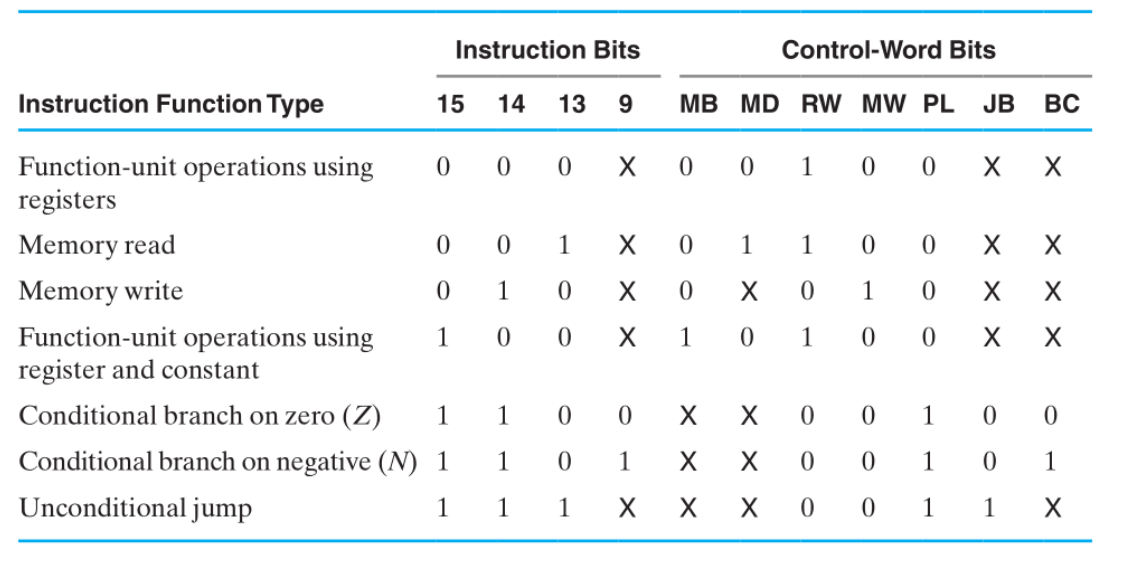
\includegraphics[scale=0.5]{assets/decoder.png}

\section{Commands}
\subsection{Commands for Data Transfer}

\begin{center}
  \begin{tabular}{ |c|c|p{8cm}| } 
  \hline
  Name & Mnemonic & Description \\ 
  \hline
  Load & LD & transfers Data from storage to a processor register \\ 
  \hline
  Store & ST & transfers data from processor register to a storage word \\ 
  \hline
  Move & MOVE & Transfers data between two registers, or between two words in storage (or one of each)  \\ 
  \hline
  Exchange & XCH & Exchanges data between two registers or two words in storage \\ 
  \hline
  Push & PUSH & Stack operation \\ 
  \hline
  Pop & POP & Stack operation \\ 
  \hline
  Stack pointer & STACKPOINTER & The register that contains the adress of the stack pointer is called SP. Points to the top element of the stack \\ 
  \hline
  Input & IN &  Moves data from/to specific registers assigned to I/O (E/A in German) \\ 
  \hline
  Output & OUT & Same thing, opposite\\ 
  \hline
  \end{tabular}
\end{center}

\subsection{Arithmetical Commands}

\begin{center}
  \begin{tabular}{ |c|c|} 
  \hline
  Name & Mnemonic  \\ 
  \hline
  Increment & INC \\
  \hline
  Decrement & DEC \\
  \hline
  Add & ADD \\
  \hline
  Subtract & SUB \\
  \hline
  Multiply & MUL \\
  \hline
  Divide & DIV \\
  \hline
  Add with carry & ADDC \\
  \hline
  Subtract with borrow& SUBB \\
  \hline
  Subtract reverse & SUBR \\
  \hline
  Negate & NEG \\
  \hline
  \end{tabular}
\end{center}

\subsection{Logical Commands}
\begin{center}
  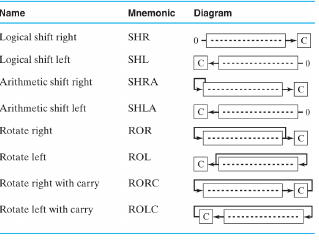
\includegraphics{assets/shiftoperations.png}
\end{center}
\subsection{Control Commands}
\begin{center}
  \begin{tabular}{ |c|c|} 
  \hline
  Name & Mnemonic  \\ 
  \hline
  Branch & BR \\
  \hline
  Jump & JMP \\
  \hline
  Call Procedure & CALL \\
  \hline
  Return from Procedure & RET \\
  \hline
  Compare (by subtraction) & CMP \\
  \hline
  Test(by ANDing) & TEST \\
  \hline
  \end{tabular}
\end{center}
\subsection{Conditioned Jump Commands}
Uses the flags of the ALU

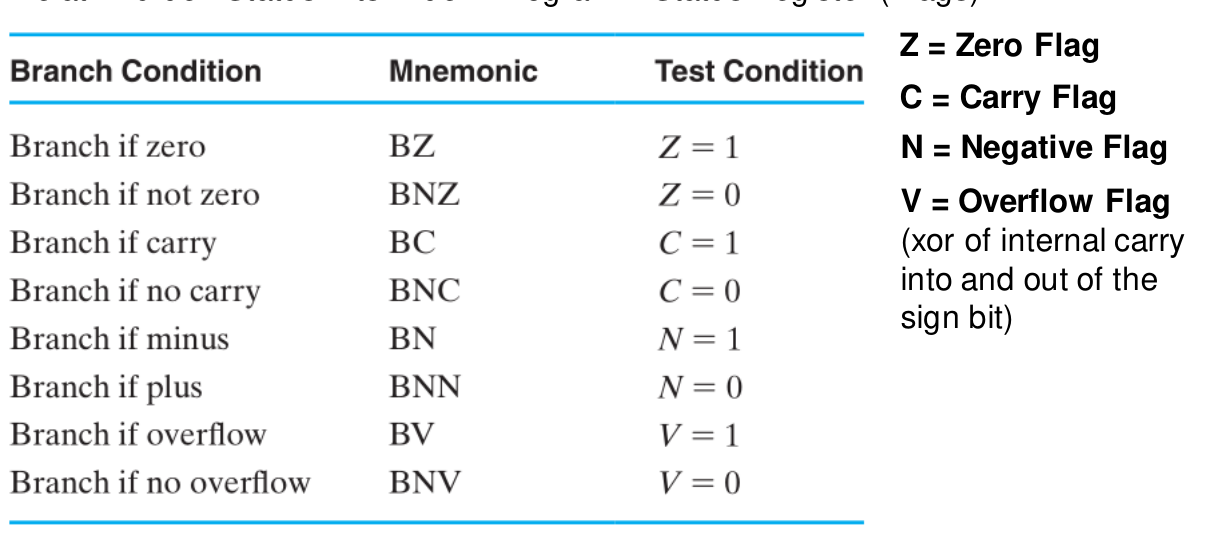
\includegraphics[scale=0.5]{assets/conditionedjumps.PNG}

\section{Pipelining a processor data path}
\subsection{Pipelined Data Path}
This process inserts flip flops in the middle of a data path, to allow for a 'reset'. This reduces the length of the largest path (and its time), allowing for the  clock to run faster, which ends up making a processor faster.

We have two important concepts regarding this
\begin{itemize}
  \item Latency: Amount of time to process a command
  \item Throughput: Number of commands that can be executed in a measure of time
\end{itemize}

\subsubsection{Three Step Pipelining}
\begin{enumerate}
  \item Operand Fetch (OF)
  \item Execution (EX)
  \item Write Back (WB)
\end{enumerate}

This makes so that in a pipeline, at a certain step, there is one instruction in the OF step, another instruction in the EX step, and another in the WB step.

\subsubsection{Four Step Pipelining}
\begin{enumerate}
  \item Instructin Fetch (IF)
  \item Decode and Operand Fetch (DOF)
  \item Execution (EX)
  \item Write Back (WB)
\end{enumerate}


As expected, there can be some hazards of working like this

\subsection{Pipeline Hazards}
Hazards are problems at the clock cycle level that arise when an
operation within a pipeline is delayed by one or more clock cycles
relative to the time at which the instruction for the
operation was fetched.


Types of hazards:
\begin{itemize}
  \item Data hazards: occur when a subsequent instruction attempts to use the
result of the operation before it has been calculated. Old
values lead to incorrect results.
 \item Control hazards: occur during program branches.
\end{itemize}

\subsubsection{Data Hazards}

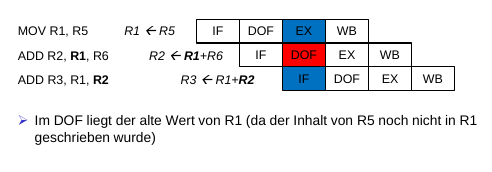
\includegraphics[]{assets/datahazard.png}
 
Pretty self explanatory how they happen

\paragraph{Software Solution: } Make the compiler analize the instructions, and if we see one of those overwriting will happen, add as many NOP (No-Operation) as needed so that they act as a blank buffer to avoid this

The issues with this is that the compiler has to handle it by itself, and that it makes the code longer

\paragraph{Hardware Solution: }If an operand is identified within the DOF stage that has not yet been
written back, the associated execution of the EX
phase and the write-back phase of the instruction is delayed by delaying the
pipeline flow in the IF and DOF phases is delayed for one clock cycle.


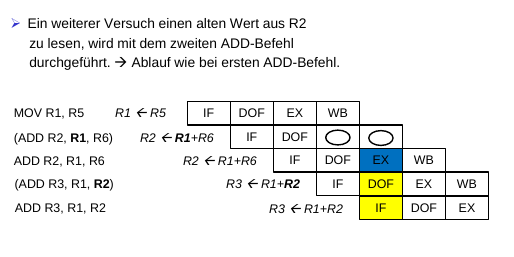
\includegraphics[]{assets/datahazard2.png}
 
\paragraph{Data Forwarding Solution: } If the edge case happens, just forward the data to where it should be. Has the disatvantage of possibly reducing a bit the latency


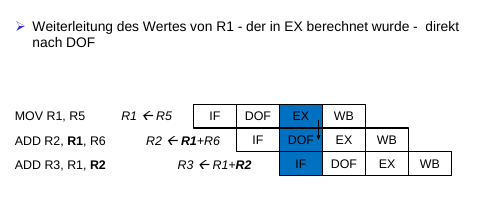
\includegraphics[]{assets/datahazard3.png}
 
\subsubsection{Control Hazards}

These hazards occur when you have branching. Because you cant know previously know where the branch will jump, it can affect pipelining.

The jump will only take place in the EX step, so until the operation gets there, we are executing operations that may affect the outcome of the code.

\paragraph{ Software Solution: } Add NOP until we evaluate the branch statement. Its an extra buffer but an easy solution.

\paragraph{ Branch Prediction Solution: } Guessing which branch it will be, if it ends up not being the correct guess, we abort the execution of the instructions already put in.

\section{Cache and storage systems}


There is something called Moore's law, that represents that the processor performance grows faster than the memory (roughly 50% gap every year)

\subsection{Memory hierarchy}

The lowest level of the hierarchy is the smallest, fastest memory, called \textbf{Cache}

So that the hierarchy works, are a big part of the CPU-Commands and Operands fetched from the cache


\[ [\text{CPU} \leftrightarrow \text{Cache}] \leftrightarrow \text{Main Memory} \leftrightarrow \text{Hard Drive}\]

The rest of the operands and CPU-Instructions are loaded from the main memory.

The cache fetches all data from the main memory

The hard drive prepares all data for the main memory.


The speed and size of memory are inversely proportional


We have two different caches
\begin{itemize}
  \item Instruction Cache
  \item Data Cache
\end{itemize}
Allows to fetch an instruction and its data in a single cycle


\subsection{Principle of Locality}
A usual program uses Loops. These loops repeat the same instructions (but with possibly differejt data)


Example: A loop repeats 8 commands 100 times.

This produces that the fetch of each of the 8 instructions must be called 100 times. THis is called \textbf{temporal locality}, which describes the effect of having a past fetch to a memmory address that will be repeated with a high likelyhood

Apart from this, there is also a high probability that the adresses of the opeands lie in sequential order. This is called \textbf{spatial locality}

\subsubsection{Locality of Reference - Principle of Locality}
\begin{itemize}
  \item Reference: Describes a reference to memory adress for command access and read/writing operands
  \item Locality: Refers to relative points in time (temporal locality) at which commands and operands are accesed, as well as relative positions in the main memory (spatial locality)
  \item If an element has been referenced, there is an increased proability of repetition of access
  \item Spatial locality: If an element has been accessed, increased probability of nearby elements being accessed
\end{itemize}

\paragraph{Operands: } A typical program contains array. They both affect temporal and spatial localities.

\subsection{Cache and memory hierarchy}
Objecive: Make the most use of locality


\begin{itemize}
  \item Use caches for faster access
  \item \textbf{Cache hit: } The data we are searching for is in the small, fast memory (\textbf{Low Latency Access})
  \item \textbf{Cache miss: } Data is in the main memory. (\textbf{High Latency Access (DRAM)})
\end{itemize}

\subsubsection{Characteristics of the Memory Hierarchy}

\begin{enumerate}
  \item Level 1: KB -- (L1 Cache) -- Smallest information unit: 4-8 Bytes (word)
  \item Level 2: MB -- (L2 Cache) -- Smallest information unit: 8-32 Bytes (Block)
  \item Level 3: GB -- (Main Memory) -- Smallest information unit: 1-4 Blocks
  \item Level 4: TB -- (Secondary Memory) -- Smallest information unit: 1024+ Bytes (disk sector)
\end{enumerate}

The cost per byte is highest at Level one and cheapest at Level 4

\subsubsection{Caches}
Caches use both types of predictability to store their data. Both spatial and temporal locality are used.


L1 Cache is divided in Data Cache and Instruction Cache. Both L1 and L2 caches are found in the main proccessor

\paragraph{Terminology: Hit and Miss Rate: } A hit is defined as the data being found in the upper level memory (Block X)

\textbf{Hit Rate: } Amount of memory accesses in upper level memory

\textbf{Hit time: } Access time in upper level = Data access time + time to decide hit/miss 

\textbf{Miss: } Data isn't found in the upper level memory and must be fetched in the lower level memory.

\begin{itemize}
  \item Miss Rate = 1- Hit rate
  \item Miss Penalty: Time necessary to make a switch in the upper level memory + time to send the data block 
  
  Hit Time <<< Miss Penalty
\end{itemize}

\subsubsection{Direct Mapped Cache}
Its a method to find a memory address for data in the cache. This method directly uses the address of the word in main memory

Each storage address maps to an cache address.

Address assignment
\begin{itemize}
  \item Cache Index: Memory Address $\mod$ Nº blocks in cache
  \item Cache Tag: Memory Address without the index digits
\end{itemize}

\subsubsection{Fully Associative Cache}

Each memory location can be mapped to any of the eight addresses within the cache. 

The tag describes the complete word address in the main memory

Searching the cache for tags to locate a data word can be expensive


\subsubsection{Associative Memory for 4-Bit tags}



STILL TODO. NOT UNDERSTANDING EVERYTHING







\end{document}

